\chapter{Notification System}
\label{kapitel_ampelsystem}

\section{General}

The notification system is a reminder and confirmation system which can be used for students, lecturers and staff.
When the user logs in, their open notifications will be displayed in the title bar as red or yellow traffic lights based on their urgency (see Figure \ref{ampel_icons}).
Administrators can create and manage new notifications.

\begin{figure}
	\centering
	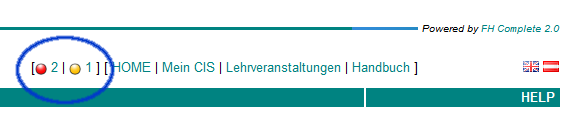
\includegraphics[width=0.70\textwidth]{CIS_Ampelsystem_Ampelicons.png}
	\caption{Notifications are displayed in the title bar as red or yellow traffic lights}
	\label{ampel_icons}
\end{figure}

Clicking on a traffic light will open an overview page where each notification can now be confirmed individually (see Figure \ref{ampel_uebersicht}).
A notification can be limited by the following parameters:
\begin{description}

	\item[Description:] Title and contents of the notification.
	\item[Target Group:] It is possible to define exactly who should receive a notification. Notifications can be displayed for defined groups of people (staff, students, ...) and/or individuals.
	\item[Deadline:] Specifies the date when a notification will be considered "`overdue"'. The traffic light will turn "`red"' on this date.
	\item[Lead Time (in days):] Specifies the date when a notification will be displayed as a "`yellow"' traffic light.
	\item[Expiration Time (in days):] Specifies when a notification will no longer be displayed. It does not matter if the notification has been confirmed or not.
\end{description}

\begin{figure}
	\centering
	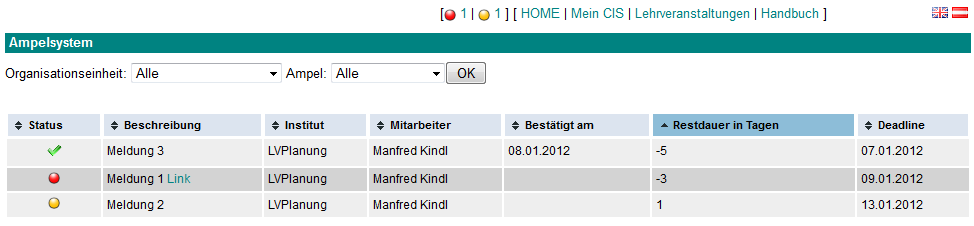
\includegraphics[width=1\textwidth]{CIS_Ampelsystem_Ampeluebersicht.png}
	\caption {Overview of the notification confirmation page}
	\label{ampel_uebersicht}
\end{figure}

\section{Overview of the Notifications}
\label{ampeluebersicht}

As can be seen in Figure \ref{ampel_uebersicht}, all the notifications are listed on the overview page. Notifications before the deadline are marked with a yellow traffic light, notifications that have exceeded the deadline are marked with a red traffic light and confirmed notifications are marked with a green check mark.
When a notification reaches the expiration date, it is no longer displayed (it does not matter whether it has been confirmed or not).

\subsection{Confirming a Notification}

To confirm a notification, click on "`Confirm"' in the last column. The notification will then be marked with a green check mark and will continue to be displayed as "`confirmed"' until the expiration date.

\section{Other}

You can sort the list by clicking the column headings.

\section{Overview of the Notifications for Heads of Departments}
\label{ampeluebersicht_leiterinnen}

If you have the appropriate user rights, you can view the status of all the notifications under "`My CIS -> Notification Overview"'.
This will provide you with an overview of exactly who has confirmed a notification or not.
You can filter the list according to organizational unit and/or traffic light descriptions and sort them by clicking the column headers.

The date on which a notification was confirmed can be seen in the column "`Confirmed on"'.
The column "`Remaining time in days"' displays how many days are remaining until the notification reaches the deadline, or in the case of negative numbers, the number of days by which the deadline has been exceeded.
